\documentclass{article}
\usepackage[utf8]{inputenc}
\usepackage[top=2cm, bottom=4.5cm, left=2.5cm, right=2.5cm]{geometry}
\usepackage{graphicx}
\title{ANLY601 Assignment1}
\author{Shaoyu Feng (sf865) \\
Collobrator: Mengtong Zhang \\
Collobrator: Yunjia Zeng 
}

\date{January 2020}

\begin{document}

\maketitle

\section{Fundamentals and Review}
\begin{enumerate}
\item \textbf{Exercise 1 (Likelihood Estimation)} \\
1. What is the maximum likelihood estimate for $\theta$ when $X_i$  $\sim$  Geometric($\theta$)? \\ \\ 
\textbf{Ans}:
The likelihood function for geometric distribution is given by $L(\theta)=\theta^n(1-\theta)^{\sum_1^n(x_i)-n}$.\\
Take the log of the likelihood function: $ln(L(\theta))=nln(\theta)+(\sum_1^n x_i-n)ln(1-\theta)$. 
Take the derivative of the log likelihood function, and let it equal to 0, we have: 
$$\frac{d(ln(L(\theta)))}{d\theta}=\frac{n}{\theta}-\frac{\sum_1^n x_i-n}{1-
\theta}=0$$
$$\theta=\frac{n}{\sum_1^n x_i}$$。 
Therefore the maximum likelihood esimation for $\theta$ for geometric distribution is $\frac{1}{X}$ \\

2. What is the maximum likelihood estimate for a and b when $X_i$ $\sim$ Unif (a, b)? \\ \\ 
\textbf{Ans}:
The likelihood function for uniform distribution with a, b is: 
$$ L(a,b)=\frac{1}{(b-a)^n}$$ 
Take the natural log for this likelihood function: 
$$ln(L(a,b))=-nln(b-a)$$
Take the derivative with respect to a and b respectively: 
$$\frac{d}{da}ln(L(a,b))=\frac{n}{b-a}$$
$$\frac{d}{db}ln(L(a,b))=\frac{-n}{b-a}$$ 
We can see that the derivative with respect to a is monotonically increasing, So we take the largest a possible which is $a_{MLE}=min(x_i)$. Similarly, We can see that the derivative with respect to b is monotonically decreasing, So we take the smallest possible of b which is $b_{MLE}=max(x_i)$.\\

\item \textbf{Exercise 2 (Loss Function)} \\

1. Show that squared error loss (L2 loss) is equivalent to the negative log likelihood of a Y $\sim$ N($\mu,\sigma^2$) where $\sigma$ is known. \\ \\ 
\textbf{Ans}: \\
Log likelihood for Gaussian is given  by: 
$$
LL=\sum_{n=1}^Nlog(N(x_n|\mu,\sigma^2) \\
=\sum_{n=1}^Nlog(\frac{1}{\sqrt{2\pi\sigma^2}}e^{-\frac{1}{2}}\frac{(x_n-\mu)^2}{\sigma^2})
$$
we then have 
$$
LL=\sum_{n=1}^N(-log(\sqrt{2\pi\sigma^2}) + (-0.5)\frac{(x_n-\mu)^2}{\sigma^2})
$$
$$
LL=-\frac{N}{2}log(2\pi\sigma^2)-\frac{1}{2\sigma^2}\sum_{n-1}{N}(x_n-\mu)^2
$$
From above notation, we can easily see that the negative log likelihood of a Gaussian is same with L2 Loss (given $\sigma$ is a constant).

2. Show that the mean absolute error (L1 loss) is equivalent to the negative log likelihood of a Y $\sim$ LaPlace($\theta$) \\ \\
\textbf{Ans}: \\
Log likelihood for Laplace isgiven by: 
$$LL=\sum_{n=1}{N}log(L(x_n|\mu,\theta))=\sum_{n=1}^{N}\frac{1}{2\theta}e^(-\frac{|x-\mu|}{\theta}))$$
$$LL=-Nlog(2\theta)-\frac{1}{b}\sum_{n=1}^{N}|x-\mu|$$

Similarly, we can see that L1 loss is equivalent to negative log likelihood of Laplace($\theta$)

\item \textbf{Exercise 3 (Decision Rules)} \\
Suppose that X has mean $\mu$ and variance $\sigma^2 < \infty$ show that: \\

1. Show that the mean is optimal decision rule for the mean squared error when the decision rule is unbiased \\ \\
\textbf{Ans}: \\

For mean square error, loss is written as : $$
L(\theta,\delta(X))=E[(\theta-\delta(X))^2]=VAR(\delta(X))+E(\delta(X)-\theta)^2
$$
If the decision rule is unbiased, the second terms on the right hand side is 0, we can simply choose mean value as a decision rule to minimize the loss. \\

2. Show the median is the optimal decision rule for the mean absolute error. \\
\textbf{Ans}: \\
To minimize $E(|X-a|)$, we see that 
$$E|X-a|=\int_{-\infty}^{\infty}|x-a|f(x)dx = \int_{-\infty}^{a}-(x-a)f(x)dx + \int_{a}^{\infty}(x-a)f(x)dx $$
$$=\int_{-\infty}^{a}f(x)dx -\int_{a}^{\infty}f(x)dx
$$
In order to minimize such loss, we can choose a as median as it will make the loss to be 0. \\


\item \textbf{Exercise 4 (Convexity)} \\ 
Suppose Y $\sim$ Bernoulli(p) where p = 1/(1 + exp(-$\beta$x)) For a fixed x show that:\\ 
1. The cross entropy loss $L(y,p)=-(ylog(p))+(1-y)log(1-p))$ is convex with respect to $−\beta$. \\
\textbf{Ans}: \\
First order derivative of the loss function is given by: 
$$\frac{dL}{d\beta}=\frac{dL}{dp}*\frac{dp}{d\beta}=-(\frac{y}{p}-\frac{1-y}{1-p})*(\frac{\beta e^{-\beta x}} {(e^{-\beta x}+1)^2})$$
Second order derivative is given by: 
$$
\frac{d^2L}{d\beta^2}=\frac{x^2 e^{\beta x}}{(e^{\beta x}+1)^2}
$$
For the second order derivative, we can see that for a fixed x, the results is always bigger or equal to 0, which satisfies second order theorem of convexity. Thus we say the cross entropy loss is convex with respect to $−\beta$.


2. The mean squared error loss L(y, p) = (y − p)$^2$ is not convex in $−\beta$ \\
\textbf{Ans}: \\
First order derivative of the loss function is given by: 
$$\frac{dL}{d\beta}=\frac{dL}{dp}*\frac{dp}{d\beta}=-2(y-p)p(1-p)x$$
Second order derivative is given by: 
$$
\frac{d^2L}{d\beta^2}=-2[y-2yp-2p+3p^2]x^2p(1-p)
$$
This does not satisfy second order convexity. One counter example is that when y=0, the second order derivative is positive only when p is in range [0, 2/3], this disprove the convexity of Mean squared loss. 

\item \textbf{Exercise 5 (decision Boundary)} \\ 
\textbf{Ans}: \\
For part2, the logit for $f_\theta(x)$ with different parameter is given by: \\
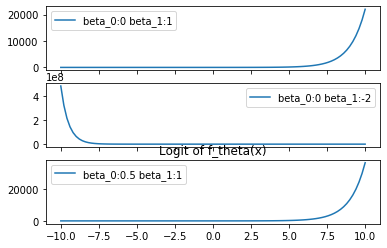
\includegraphics[width=10cm, height=10cm]{Assign1plot1.png} \\
We have $logit(f_\theta(x))=log(\frac{f_\theta(x)}{1-f_\theta(x)})=log(\frac{1}{exp(-\beta x)})=\beta x$. Logit function is a monotonous function, we can say that $\theta x=\theta_0+\theta_1x$ is a linear seperating hyperplane. 

  

\end{enumerate}
\section{Parametric learning}
\begin{enumerate}
\item \textbf{Exercise 6 (Sufficient Statistic))} \\
Suppose $X_{i=1}^{N} \sim N(\mu,\sigma^2), \sigma < \infty$ and is known. Show that the sample mean T(X) = $\bar X $ is a sufficient statistic for $\mu$. \\
\textbf{Ans}: \\

Based on the Factorization Theorem, let $f(x|\theta)$ denote the joint pdf or pmf of a sample X. A statistic is a sufficient statistic for $\theta$ if and only if there exists a factorization of the function $f(x|\theta)$ into two functions, h(x) and $g(t|θ)$ for all sample points x and all parameter points θ: $f(x|\theta)=g(T(x)|\theta)h(x)$. \\

In this case, we know the population follows normal with known variance, we have: 
$$
f(x_1,...,x_n|\mu)=(2\pi)^{-n/2}\sigma^{-n}exp^{(\frac{-1}{2\sigma^2}\sum_{i=1}^{n}(x_i-\mu)^2)}
$$
$$
=(2\pi)^{-n/2}\sigma^{-n}exp^{(\frac{-1}{2\sigma^2}\sum_{i=1}^{n}x_i^2+\frac{\mu}{\sigma^2}\sum_{i=1}^{n}x_i-\frac{n\mu^2}{2\sigma^2})}
$$
Since $\sigma^2$ is known, we let: 
$$ h(x)= 2\pi)^{-n/2}\sigma^{-n}exp^{(\frac{-1}{2\sigma^2}\sum_{i=1}^{n}x_i^2}$$ 
and 
$$
g(r(x_1,x_2,...,x_n),\mu)=exp^{\frac{\mu}{\sigma^2} r(x_1,x_2,...,x_n)-\frac{n\mu^2}{2\sigma^2}}
$$
where 
$$
r(x_1,x_2,...,x_n)=\sum_{i=1}^{n}x_i
$$
By the factorization theorem this shows that $\sum_{i=1}^{n}x_i$ is a sufficient statistics, It follows that the sample mean is also a sufficient statistic. \\

\item \textbf{Exercise 7 (Ancilliarity)} \\
Let ${X_i}^n_{i=1}$ be independent and identically distributed observations from a location parameter family with cumulative distribution function $F(x - \theta)$. Show that range of the distribution of $R = max_i(X_i)-min_i(X_i)$ does not depend on the parameter $\theta$. \\ 
\textbf{Ans}: \\

Given the fact that $X_i$ is an independent and identically distributed observations from a location parameter family. we then have the fact that$X_1 = Z_1+\theta, ..., X_n= Z_n + \theta$ and $min_i(X_i) = min_i(Z_i + \theta), maxi(Xi) = max_i(Z_i + \theta)$, where ${Z_i}^n_{i=1}$ are independent and identically distributed observations from F(x). \\
In such a case, we say that $R = max_i(X_i)-min_i(X_i)=max(Z_i)-min(Z_i)$ is also location invariant, this means that $R = max_i(X_i)-min_i(X_i)$ is ancillary and thus does not depend on  the parameter $\theta$. \\

\item \textbf{Exercise 8 (Completeness)} \\
Show that $N(\mu,\mu^2)$ has a sufficient statistic but is not complete. \\
\textbf{Ans}: \\
We have $$
f(x_1,...,x_n|\mu)=(2\pi)^{-n/2}\mu^{-n}exp^{(\frac{-1}{2\mu^2}\sum_{i=1}^{n}(x_i-\mu)^2)}
$$
$$
=(2\pi)^{-n/2}\mu^{-n}exp^{(\frac{-n}{2|\mu|}(x_i-\mu)^2)}exp^{-\frac{s^2}{2\mu^2}}
$$
It is trivial to say that $(\bar x, s^2)$ is a sufficient statistic. Then we have $h(T)=\bar x^2 -\frac{n+1}{n}s^2$. 
$$
E(h(T))=E((\bar x)))^2 + Var(\bar x) -\frac{n+1}{n}E(s^2)=\mu^2+\frac{\mu^2}{n}-\frac{n+1}{n}\mu^2=0
$$
But h(T) is not travially 0 for all $\theta$


\item \textbf{Exercise 9 (Regular exponential family)} \\
 Show that the Poisson distribution is part of the regular exponential family.\\
\textbf{Ans}: \\
$f_\theta$ us said to be an exponential family if it has following form: 
$$f(x|\theta)=h(x)e^{\psi(\theta)T(X)-A(\theta)}$$ where $A(\theta)$ is the cumulant, T(X) is the sufficient statistics for the parameter. The canonical form can be rewritten as:
$$f(X=x|\eta)=h(x)^{\eta T(X)-B(\eta)}$$ 
For Poisson distribution, we have probablitue mass function given by: 
$$
p(x|\lambda)=\frac{\lambda^x e^{-\lambda}}{x!}
$$
$$
=\frac{1}{x!} e^{xlog\lambda -\lambda}
$$
In such a case, we show that poisson distribution is an exponential family distribution with $\eta=log \lambda $ and T(x)=x and $B(\eta)= \lambda $ and $h(x)=\frac{1}{x!}$

\item \textbf{Exercise 10 (Regular exponential family)} \\
\textbf{Ans}: \\
Recall that we have: 
$$B(\eta)=log \int _x h(x)e^{\eta T(X)} dx$$
Differentiating with respect to $\eta_i$ yields
$$
\frac{\delta}{\delta \eta_i}B(\eta)=\frac{\int _x T_i(x)h(x)e^{\eta T(X)} dx}{\int _x h(x)e^{\eta T(X)} dx}= E_i[T_i(X)]
$$ 
Let $Z(\eta)=\int _x T_i(x)h(x)e^{\eta T(X)}dx$, differentiating this expression again with respect to $\eta_j$, we then have: 
$$
\frac{\delta^2}{\delta\eta_i\eta_j}B(\eta)=\frac{\int _x T_i(x)T_j(x)h(x)e^{\eta T(X)} dx}{Z(\eta)}-\frac{(\frac{\delta}{\delta\eta_i})(\frac{\delta}{\delta\eta_j})}{Z(\eta)^2}
$$
$$
=E_\eta[T_i(X)T_j(X)]-E_\eta[T_i(X)]E_\eta[T_j(X)]
=Cov_\eta[T_i(X),T_j(X)]
$$

\item \textbf{Exercise 11 (Delta Method)} \\
\textbf{Ans}: \\
We have $X\sim Bernoulli(p)$, then $n\bar x$ follows binomial distribution. We then have $E(\bar x)=p$ and $var(\bar x)=np(1-p)/n^2=\frac{p(1-p)}{n}$\\
Based on Delta Method, we say that $$
Var(\bar x(1-\bar x))=(1-2p)^2 Var(\bar x)=\frac{(1-2p)^2(1-p)p}{n^2}
$$

Therefore we have approximate distribution for $\tau$ is $N(0,(1-2p)^2(1-p)p )$

\end{enumerate}

\section{Fundamentals and Review} 
\begin{enumerate}
\item \textbf{Exercise 12 (Joint Entropy)} \\
1.Compute the joint entropy H(X,Y) of X and Y. \\ 
\textbf{Ans}: \\
$$
H(X,Y)=\sum_x\sum_y P(x,y) log_2(P(X,y))$$$$
=2*1/4*log_2(1/4)+2*1/6*log_2(1/6)+2*1/12*log_2(1/12)=-2.45
$$
2. Find the Marginal distribution of X and the conditional entropy H(Y|X) \\
\textbf{Ans}: \\
Marginal Distribution for X is given by:
P(X=0)=P(X=1)=P(X=2)=1/3. \\
For conditional Entropy: 
$P(Y=0|X=0)=3/4 \\
P(Y=0|X=1)=1/4 \\
P(Y=0|X=2)=1/2 \\
P(Y=1|X=0)=1/4 \\
P(Y=1|X=1)=3/4 \\
P(Y=1|X=2)=1/2 \\ $
and Therefore: 
$H(Y|X=0)= 3/4*log_2(3/4)+1/4*log_2(1/4)=-0.81$ \\
$H(Y|X=1)= 1/4*log_2(1/4)+3/4*log_2(3/4)=-0.81$ \\
$H(Y|X=2)= log_2(1/2)=-1$ \\
$H(Y|X)=1/3*(-0.81*2-1)=-0.87$

3. Verify the entropy results above by using the chain rules that relates $H(X, Y ) to H(X) and H(Y |X)$.  \\
\textbf{Ans}: \\
$H(X)=1/3*3*log_2(1/3)=-1.58$ Therefore $H(X,Y)=H(X)+H(Y|X)$ \\

\item \textbf{Exercise 13 (Differential Entropy)} \\ 
Find the differential entropy (this is the continuous version of entropy) of a multivariate normal distribution. \\ 
\textbf{Ans}: \\
$$
Diferential Entropy=- \int _{-\infty}^{+\infty} N(x|\mu,\sum)ln(N(x|\mu,\sum))dx
=-E[ln(N(x|\mu,\sum))]
$$
$$
=-E[ln((2\pi)^{-\frac{D}{2}}|\sum|^{-0.5}e^{-0.5(x-\mu)^T\sum^{-1}(x-\mu)})]
$$
$$
=\frac{D}{2}ln(2\pi)+\frac{1}{2}ln|\sum|+\frac{1}{2}E[(x-\mu)^T\sum^{-1}(x-\mu)]
$$
we have
$$
E[(x-\mu)^T\sum^{-1}(x-\mu)]= E[tr((x-\mu)^T\sum^{-1}(x-\mu))]=tr(E[\sum^{-1}(x-\mu)(x-\mu)^T])=tr(\sum^-1\sum)=tr(I)=D
$$

$$
Diferential Entropy=\frac{D}{2}ln(2\pi)+\frac{1}{2}ln|\sum|+D 
$$
where D is the number of dimensions.




\end{enumerate}

\end{document}
